\documentclass[letter,12pt]{article}
\usepackage[letterpaper,right=1in,left=1in,top=1in,bottom=1in]{geometry}
\usepackage{setspace}

\usepackage[utf8]{inputenc}   % allows input of special characters from keyboard (input encoding)
\usepackage[T1]{fontenc}      % what fonts to use when printing characters       (output encoding)
\usepackage{amsmath}          % facilitates writing math formulas and improves the typographical quality of their output
\usepackage[hyphens]{url}     % adds line breaks to long urls
\usepackage[pdftex]{graphicx} % enhanced support for graphics
\usepackage{tikz}             % Easier syntax to draw pgf files (invokes pgf automatically)
\usetikzlibrary{arrows}

\usepackage{mathptmx}           % set font type to Times
\usepackage[scaled=.90]{helvet} % set font type to Times (Helvetica for some special characters)
\usepackage{courier}            % set font type to Times (Courier for other special characters)

\usepackage[longnamesfirst, sort]{natbib}\bibpunct[]{(}{)}{,}{a}{}{;} % handles biblio and references 

\usepackage{rotating}         % sideway tables and figures that take a full page
\usepackage{caption}          % allows multipage figures and tables with same caption (\ContinuedFloat)

\usepackage{dcolumn}          % needed for apsrtable and stargazer tables from R to compile
\usepackage{arydshln}         % dashed lines in tables (hdashline, cdashline{3-4}, 
                              %see http://tex.stackexchange.com/questions/20140/can-a-table-include-a-horizontal-dashed-line)
                              % must be loaded AFTER dcolumn, 
                              %see http://tex.stackexchange.com/questions/12672/which-tabular-packages-do-which-tasks-and-which-packages-conflict


\newcommand{\mc}{\multicolumn}

%% TO ADD NOTES IN TEXT, PUT % BEFORE THE ONE YOU WANT DISABLED
\usepackage[disable]{todonotes}                            % no show
%\usepackage[colorinlistoftodos, textsize=small]{todonotes} % show notes
\newcommand{\emm}[1]{\todo[color=red!15, inline]{\textbf{Eric:} #1}}

%% \usepackage{xr} % allows cross-ref to other file
%% \externaldocument{urge15appendix}

%% %for submission: sends figs, tables, and footnotes to last pages
%% \RequirePackage[nomarkers,nolists]{endfloat}     % sends tables and figures to the end
%% \RequirePackage{endnotes}                        % turns fn into endnotes; place \listofendnotes where you want 
%%                                                  %the endnotes to appear (it must be after the last endnote).
%% \let\footnote=\endnote
%% \newcommand{\listofendnotes}{
%%    \begingroup
%%    \parindent 0pt
%%    \parskip 2ex
%%    \def\enotesize{\normalsize}
%%    \theendnotes
%%    \endgroup
%% }

%% % for submission: drop page numbers when producing title page
%% \pagenumbering{gobble} % Remove page numbers (and reset to 1)
%% \pagenumbering{arabic}% Arabic page numbers (and reset to 1)


\setcitestyle{citesep={;}}

\begin{document}

\title{Incumbency advantage upon removal of single-term limits: Mexican municipal elections}
\author{Eric Magar \\ ITAM, Mexico City
}
\date{\today}
\maketitle

% \newpage

\begin{abstract}
\noindent En route
\newline
\newline
\textbf{Keywords}: Incumbency advantage, term limits, electoral reform, municipal elections, Mexico
\end{abstract}

% \newpage

%\doublespacing

\section{Introduction}

\noindent En route

\section{Reform, consequences}

2014 reform surprising removal of term limits. Adopted in 1934, cornerstone of partisan centralization of power under the PRI. Removed immediate reelection at all levels.

PAN placed removal among its requests, as was standard. Unlike the past, when left and PRI would veto, it was adopted along other changes.

Federal deputies can reelect for up to four consecutive three-year terms, senators for two consecutive six-year terms. Fearing that members of Congress might gain too much independence from party leaders, reformers retained some control: incumbents must be renominated by the same party in whose ticket they originally ran. Elaborate. 

Kick-off in the 2021 mid-term election.

At subnational level, reformers left some discretion to state legislatures. State law-makers: either 2-, 3-, or 4-term limits. For municipal officers single- or 2-term limits. Two states only retained single-term limits for municipal presidents, Hidalgo and Veracruz. Unelected municipal officers in Oaxaca's \emph{usos y costumbres} Party clause mandatory. Variable election calendars: incumbents on the ballot progressively. 

Bring from ITAM Schlesinger, Cain Ferejohn Fiorina, Mayhew, Jacobson, Samuels. 

\begin{figure}
  \centering
  \includegraphics[width=.85\columnwidth]{../graph/horizon-yrs.pdf} \\
  \caption{Extending the electoral horizons of municipal incumbents. Columns classify $N \approx 2,030$ municipalities according to the yearly reelection status of elected officeholders (430 municipalities with unelected indigenous governments are excluded).}\label{F:horizons}
\end{figure}

Figure \ref{F:horizons} reports relative frequencies of municipalities with different institutions since the reform. Each vertical bar accounts for 2,016 to 2,039 municipalities with elected officeholders (the variation is due to new units that were carved out in the period). Gray segments correspond to non-reformer states that kept the limits all municipalities nationwide had before 2014 in place. Veracruz, which has a large number of units, eventually joined reform states in 2020, dropping term limits for municipal officers that will be elected next year. Hidalgo now remains as the sole state banning consecutive municipal reelection. 

The light-green segments include the gradually but steadily vanishing term-limited municipal officers. This category had about 35 percent of observations in 2015, and less than 5 percent in 2018. Unlike gray segments, however, officeholders in this group remained ineligible for consecutive reelection due to reforms coming into force further down in time. None will remain by 2021. In mid-green are freshmen eligible for another term in office. This is the modal group, including nearly 50 percent of observations in 2015, and over two-thirds afterwards. They enjoyed extended horizons for the first time in decades: at the end of the three-year term, ambitious incumbents in this group could opt, unlike all predecessors, to fight and secure renomination to run for the same office. The reform inaugurated the possibility of holding what \citet{schlesinger.1966} calls \emph{static ambition}. The theoretical expectation is that such incumbents will behave systematically different from the rest. 

The first batch of returning incumbents, in darker-green segments, arrived in 2018. A total of 273 municipal presidents from 17 states secured reelection that year, and 12 more in 2019. Together, these account for 14 percent of observed municipalities, or just shy of 20 percent when population-weighted. The inaugural proportion is remarkable because the 2018 races concurred with a presidential election won by a landslide that, we will see, probably depressed reelection rates. (The large white indetermined category in 2021 will fill up when those races take place next year; it will break up in mid- and darker-green segments.)

Freshmen elected in 2015, representing nearly 50 percent of municipal officers, had a very different perspective from their predecessors, as they were not barred from running again at the end of the term.  

Members of Congress can be reelected for up to 12 consecutive years. With 3-year terms, 

Term limits sever the personalized electoral connection, collective reputation only without the personal element.

See \citet{cain.etal.1987} for argumentation.

\section{A hypothesis perhaps}

\begin{description}
  \item [Hypothesis 1:] Presidents are more likely to fast-track bills when the committee chair with jurisdiction over the bill  belongs to the president's party than otherwise.
\end{description}

\section{Incumbents running v.\ open seats}


\begin{table}
\centering
  \begin{tabular}{lcccclcccc}
         &   \mc{4}{c}{Incumbent on the ballot}    &&      \mc{4}{c}{Open seat}           \\ \cline{2-5} \cline{7-10}
In party & \%won   & \%lost   &   sum   &     (N)  && \%won  & \%lost &   sum   &      (N)\\ \hline
PAN      &   66    &   34     &   100   &   (121)  &&   39   &   61   &   100   &  (1,664)\\
PRI      &   47    &   53     &   100   &   (220)  &&   50   &   50   &   100   &  (3,548)\\
PRD      &   57    &   43     &   100   &    (89)  &&   39   &   61   &   100   &  (1,082)\\
Morena   &  100    &    0     &   100   &     (9)  &&   78   &   22   &   100   &     (18)\\
Other    &   53    &   47     &   100   &    (97)  &&   25   &   75   &   100   &    (632)\\ \hline
Overall  &   55    &   45     &   100   &   (536)  &&   44   &   56   &   100   &  (6,944)\\
  \end{tabular}
  \caption{Success and failure since 2005 with and without incumbent running. Excludes governments elected since 2017 whose terms have not concluded.}\label{T:successfail}
\end{table}

\section{Regression model}

% Table created by stargazer v.5.2.2 by Marek Hlavac, Harvard University. E-mail: hlavac at fas.harvard.edu
% Date and time: Wed, Oct 21, 2020 - 12:28:13 AM
% Requires LaTeX packages: dcolumn 
\begin{sidewaystable}[!htbp] \centering 
\resizebox{\textwidth}{!}{
\begin{tabular}{@{\extracolsep{5pt}}lD{.}{.}{-3} D{.}{.}{-3} D{.}{.}{-3} D{.}{.}{-3} D{.}{.}{-3} D{.}{.}{-3} } 
\\[-1.8ex]\hline 
\hline \\[-1.8ex] 
 & \multicolumn{6}{c}{\emph{Dependent variable:} vote share - E(vote share)} \\ 
\cline{2-7} 
%\\[-1.8ex] & \multicolumn{6}{c}{Residual} \\ 
 & \multicolumn{1}{c}{PAN} & \multicolumn{1}{c}{PRI} & \multicolumn{1}{c}{Left} & \multicolumn{1}{c}{PAN} & \multicolumn{1}{c}{PRI} & \multicolumn{1}{c}{Left} \\ 
\\[-1.8ex] & \multicolumn{1}{c}{(1)} & \multicolumn{1}{c}{(2)} & \multicolumn{1}{c}{(3)} & \multicolumn{1}{c}{(4)} & \multicolumn{1}{c}{(5)} & \multicolumn{1}{c}{(6)}\\ 
\hline \\[-1.8ex] 
 vote share (lagged) & -0.216^{***} & -0.051^{***} & -0.303^{***} & -0.260^{***} & -0.049^{***} & -0.210^{***} \\ 
  & (0.011) & (0.013) & (0.013) & (0.013) & (0.014) & (0.014) \\ 
  & & & & & & \\ 
 party incumbent & 0.237^{***} & 0.173^{***} & -0.077^{***} & 0.217^{***} & 0.171^{***} & -0.033^{*} \\ 
  & (0.013) & (0.014) & (0.019) & (0.013) & (0.013) & (0.017) \\ 
  & & & & & & \\ 
 other-party incumbent & -0.014 & -0.007 & 0.062^{***} & -0.021^{**} & -0.009 & 0.072^{***} \\ 
  & (0.010) & (0.009) & (0.010) & (0.010) & (0.009) & (0.009) \\ 
  & & & & & & \\ 
 party open seat & 0.176^{***} & 0.123^{***} & 0.087^{***} & 0.182^{***} & 0.125^{***} & 0.118^{***} \\ 
  & (0.005) & (0.004) & (0.006) & (0.004) & (0.003) & (0.005) \\ 
  & & & & & & \\ 
 concurrent gub. race & 0.027^{***} & 0.013 & 0.068^{***} & 0.031^{***} & -0.002 & 0.133^{***} \\ 
  & (0.010) & (0.009) & (0.014) & (0.010) & (0.009) & (0.014) \\ 
  & & & & & & \\ 
 governor & -0.017^{***} & 0.027^{***} & 0.010 & 0.012^{**} & 0.024^{***} & 0.040^{***} \\ 
  & (0.005) & (0.004) & (0.006) & (0.005) & (0.004) & (0.007) \\ 
  & & & & & & \\ 
 population (log, 10k) & -0.005^{***} & -0.004^{***} & -0.003^{***} & -0.001 & -0.001 & -0.009^{***} \\ 
  & (0.001) & (0.001) & (0.001) & (0.001) & (0.001) & (0.001) \\ 
  & & & & & & \\ 
 sd elevation (pop. weigthed) & -0.008 & -0.063^{***} & 0.041^{***} & 0.036^{**} & 0.010 & 0.045^{***} \\ 
  & (0.015) & (0.014) & (0.016) & (0.016) & (0.015) & (0.016) \\ 
  & & & & & & \\ 
 post reform & 0.077^{***} & -0.157^{***} & -0.114^{***} & 0.075^{***} & -0.159^{***} & -0.114^{***} \\ 
  & (0.005) & (0.005) & (0.006) & (0.005) & (0.005) & (0.006) \\ 
  & & & & & & \\ 
 Constant & 0.020 & 0.015 & -0.051^{***} & -0.088^{***} & 0.022 & 0.066^{**} \\ 
  & (0.013) & (0.014) & (0.013) & (0.026) & (0.025) & (0.026) \\ 
  & & & & & & \\ 
\hline \\[-1.8ex] 
 Fixed state effects & \multicolumn{1}{c}{No} & \multicolumn{1}{c}{No} & \multicolumn{1}{c}{No} & \multicolumn{1}{c}{Yes} & \multicolumn{1}{c}{Yes} & \multicolumn{1}{c}{Yes} \\
\hline \\[-1.8ex] 
Observations & \multicolumn{1}{c}{8,310} & \multicolumn{1}{c}{8,310} & \multicolumn{1}{c}{8,310} & \multicolumn{1}{c}{8,310} & \multicolumn{1}{c}{8,310} & \multicolumn{1}{c}{8,310} \\ 
R$^{2}$ & \multicolumn{1}{c}{0.221} & \multicolumn{1}{c}{0.294} & \multicolumn{1}{c}{0.112} & \multicolumn{1}{c}{0.293} & \multicolumn{1}{c}{0.344} & \multicolumn{1}{c}{0.241} \\ 
%Adjusted R$^{2}$ & \multicolumn{1}{c}{0.221} & \multicolumn{1}{c}{0.294} & \multicolumn{1}{c}{0.111} & \multicolumn{1}{c}{0.290} & \multicolumn{1}{c}{0.341} & \multicolumn{1}{c}{0.238} \\ 
Residual Std. Error & \multicolumn{1}{c}{0.162} & \multicolumn{1}{c}{0.151} & \multicolumn{1}{c}{0.171} & \multicolumn{1}{c}{0.155} & \multicolumn{1}{c}{0.146} & \multicolumn{1}{c}{0.159} \\ 
F Statistic & \multicolumn{1}{c}{262.2$^{***}$} & \multicolumn{1}{c}{384.9$^{***}$} & \multicolumn{1}{c}{116.3$^{***}$} & \multicolumn{1}{c}{90.3$^{***}$} & \multicolumn{1}{c}{114.4$^{***}$} & \multicolumn{1}{c}{69.1$^{***}$} \\ 
\hline 
\hline \\[-1.8ex] 
\textit{Note:}  & \multicolumn{6}{r}{$^{*}$p$<$0.1; $^{**}$p$<$0.05; $^{***}$p$<$0.01} \\ 
\end{tabular} 
}
  \caption{Models} 
  \label{} 
\end{sidewaystable}





\section{Discussion}

\begin{figure}
  \centering
    \caption{Population-weigthed altitude deviations in municipalities}\label{F:avgMg}
    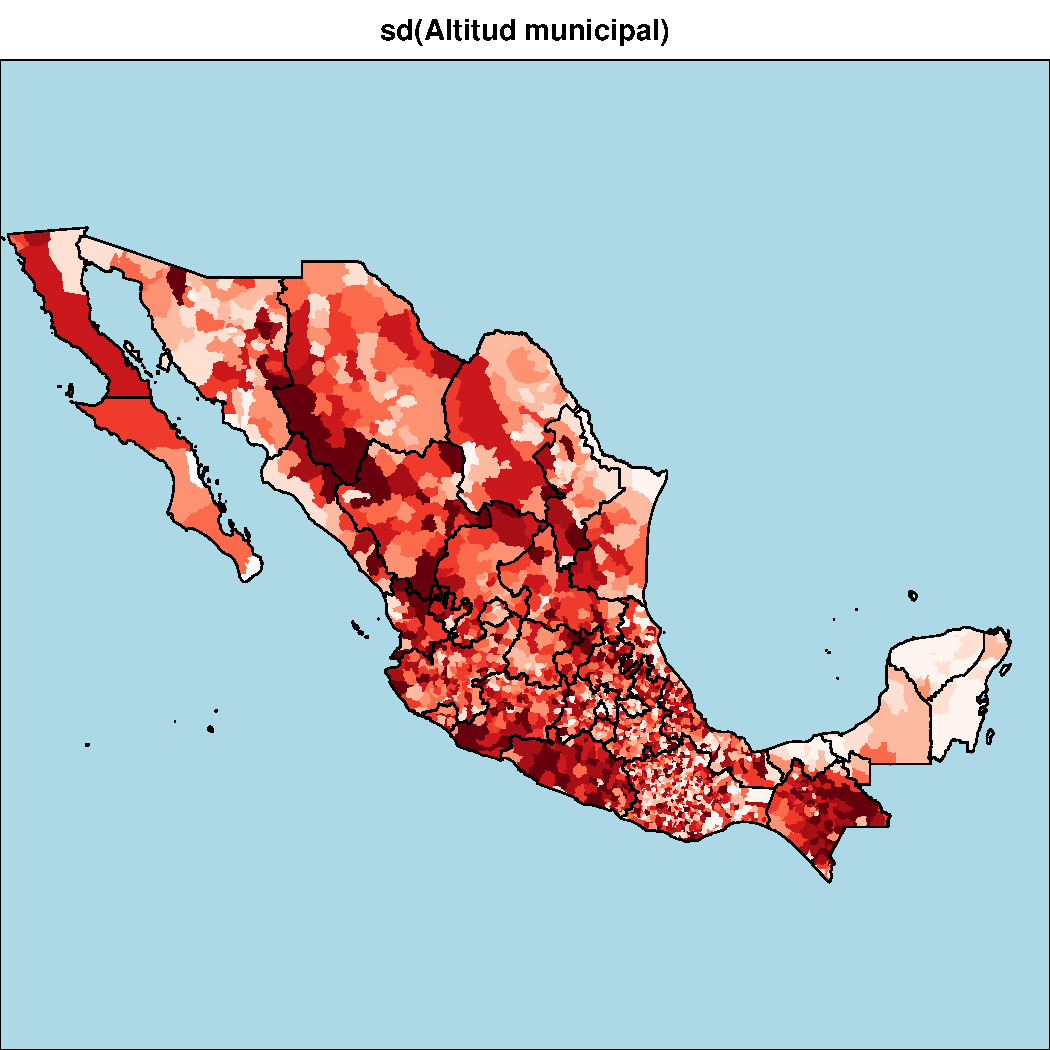
\includegraphics[width=.8\columnwidth]{../graph/map.png}
\end{figure}


\section*{Acknowledgements}
The author received financial support from the Asociaci\'on Mexicana de Cultura \textsc{a.c.}. He is responsible for mistakes and shortcomings in the study.

%% \listofendnotes

\bibliographystyle{apsr}
%\bibliography{../bib/magar}
\bibliography{/home/eric/Dropbox/mydocs/magar}

\end{document}

